\Subhead{4.10.1}{Взаимодействие света со звуком. Дифракция Брэгга и Рамана--Ната}

Акустическая деформация меняет оптическую непроницаемость через фотоупругость:
\begin{equation}
 \Delta(\varepsilon_r^{-1})_{ij}=p_{ijkl}S_{kl}.
\end{equation}
Бегущая волна образует движущуюся фазовую решётку с $\bm K$ и $\Omega$. Для дифрагированного света
\begin{equation}
 \omega_d=\omega_i\pm\Omega,\qquad \bm k_d=\bm k_i\pm\bm K.
\end{equation}
Частотный сдвиг следует из движения решётки; в кристалле волновые поверхности разных поляризаций требуют векторного построения, и простая изотропная формула угла не универсальна.

Параметр Клейна–Кука $Q_{\rm KN}=2\pi\lambda_0L/(n\Lambda^2)$ сравнивает накопленную дифракционную расстройку с толщиной взаимодействия. При $Q_{\rm KN}\ll1$ и умеренной фазовой модуляции тонкая решётка даёт режим Рамана–Ната: много порядков, а разложение $\exp[\ii v\cos(Kx-\Omega t)]$ даёт эффективности $\eta_m=J_m^2(v)$, $v=2\pi\Delta n L/\lambda_0$. При сильной модуляции условие тонкой решётки нужно проверять для значимых высоких порядков.

При $Q_{\rm KN}\gg1$ и настройке угла выделяются два связанных порядка — режим Брэгга. В изотропной среде внутренний угол $\sin\theta_B=\lambda_0/(2n\Lambda)$. При точном синхронизме, отсутствии потерь и заданной звуковой накачке связанные оптические амплитуды обмениваются энергией:
\begin{equation}
 a'_0=\ii\kappa a_1,\quad a'_1=\ii\kappa^*a_0,
 \qquad \eta_1=\sin^2(|\kappa|L).
\end{equation}
При фазовой расстройке $\Delta k$ максимум обмена уменьшается: $\eta_1=|\kappa|^2\sin^2(gL)/g^2$, $g^2=|\kappa|^2+(\Delta k/2)^2$. Высокая эффективность не требует многих порядков; она достигается полным двухволновым обменом.
\begin{center}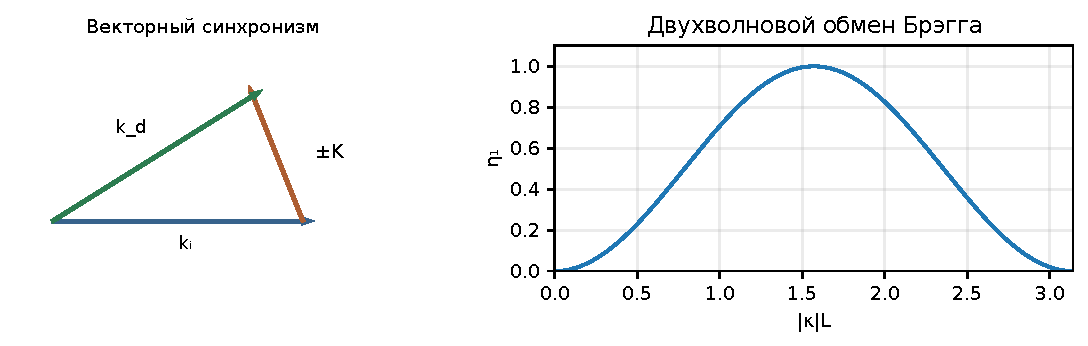
\includegraphics[width=0.87\linewidth]{figures/acoustooptic.pdf}\end{center}

